\documentclass[UTF8,a4paper,12pt]{ctexart}
\usepackage{thesis-style}
\usepackage{amsmath}

\graphicspath{{../../outputs/homework11/}}
\headermark{《金融经济数据挖掘》作业十一报告}
\reporttitle{《金融经济数据挖掘》实验报告}
\reportsubtitle{作业十一：银行信用评分模型与违约风险预测}
\author{丁致宇}
\studentid{202331060205}
\major{数据科学与大数据技术}
\phone{18765788600}
\date{2026年6月}

\begin{document}

\maketitle

\begin{ustcabstract}
本报告围绕作业十一“银行信用评分模型”展开，基于阿里天池违约贷款数据集（ID:140861）构建消费金融用户违约风险预测与标准化信用评分卡。实验以 80 万条训练样本和 20 万条测试样本为基础，完成数据加载、缺失值审计、字段清洗、类别编码、相关性分析、WOE/IV 特征筛选、逻辑回归建模、AUC/KS 评估、信用分转换、信用等级划分和用户信用提升建议输出。

本次修复重点解决了三个影响交付质量的核心问题：第一，将建模训练集与验证集提前隔离，确保类别映射、中位数填充、相关性筛选、IV 计算、WOE 分箱和标准化参数均只在训练侧拟合，避免验证集信息泄露；第二，修正信用分公式方向，采用 $Score=Offset+Factor\ln((1-p)/p)$，保证信用分越高违约概率越低；第三，将评分卡从单纯的特征系数表升级为“特征分箱--WOE--IV--分箱分数”的标准评分规则表。最终模型验证集 AUC 为 0.7058，KS 为 0.3006，5 折交叉验证 AUC 为 0.7072，信用分与违约概率相关系数为 -0.9961，评分方向和业务解释一致。
\end{ustcabstract}
\keywords{信用评分；违约风险；WOE/IV；逻辑回归；评分卡；AUC；KS}

\clearpage
\tableofcontents
\clearpage

\section{实验要求理解与总体设计}

作业十一要求建立面向消费金融用户的信用评分模型，核心交付物包括完整可运行的 Python 源代码、特征重要性可视化图表、标准化信用评分规则或评分卡，以及实验报告。该任务本质上不是追求黑箱模型的最高精度，而是要求兼顾风控场景的可解释性、稳定性和可落地性。因此，本实验选择逻辑回归作为核心分类模型，并引入金融风控中常用的 WOE/IV 特征筛选与分箱评分卡方法。

实验流程设计如图式逻辑所示：首先读取训练集和测试集，并进行目标变量分布、缺失值和数据规模审计；随后完成字段清洗、日期特征提取、类别编码和缺失值填充；接着基于建模训练集进行相关性筛选和 IV 筛选，保留具有有效区分能力的特征；最后对入模特征进行 WOE 分箱转换，训练逻辑回归模型，并将模型输出的违约概率转换为 300--850 分的信用评分。

为保证结果可复现，全部参数集中在脚本顶部配置区，核心参数如表 \ref{tab:params} 所示。完整运行入口为：

\begin{CodeBlock}
python homework11/homework11_credit_scorecard.py
\end{CodeBlock}

\begin{table}[H]
    \centering
    \caption{实验核心参数设置}
    \label{tab:params}
    \begin{tabular}{ll}
        \toprule
        参数 & 取值与说明 \\
        \midrule
        RANDOM\_SEED & 42，保证数据划分与可视化抽样可复现 \\
        TEST\_SIZE & 0.2，验证集比例 \\
        CV\_FOLDS & 5，交叉验证折数 \\
        IV\_THRESHOLD & 0.02，入模特征最低 IV 阈值 \\
        CORR\_THRESHOLD & 0.8，高相关特征剔除阈值 \\
        WOE\_BINS & 10，连续特征分箱数量 \\
        BASE\_SCORE & 600，信用评分基准分 \\
        PDO & 50，坏账赔率翻倍对应分值变化 \\
        BASE\_ODDS & 1，600 分对应中性好坏比 \\
        SCORE\_MIN / SCORE\_MAX & 300 / 850，信用分上下限 \\
        \bottomrule
    \end{tabular}
\end{table}

\section{数据来源与探索性分析}

\subsection{数据来源与字段结构}

实验数据来自阿里天池公开违约贷款数据集，训练集文件为 \path{data/homework11/train.csv}，测试集文件为 \path{data/homework11/testA.csv}。训练集包含目标变量 \texttt{isDefault}，测试集不包含目标变量，用于输出最终信用分和违约概率预测。

\begin{table}[H]
    \centering
    \caption{数据规模摘要}
    \label{tab:data-scale}
    \begin{tabular}{lrr}
        \toprule
        数据集 & 样本数 & 字段数 \\
        \midrule
        训练集 & 800,000 & 47 \\
        测试集 & 200,000 & 46 \\
        \bottomrule
    \end{tabular}
\end{table}

字段主要分为四类：个人基础信息、负债信息、征信行为信息和贷款申请信息。其中，\texttt{annualIncome}、\texttt{dti}、\texttt{ficoRangeLow}、\texttt{loanAmnt}、\texttt{subGrade} 等变量具有明确金融风控含义，是信用评分模型的重要候选特征。

\subsection{目标变量分布}

训练集中正常还款样本 640,390 条，占比 80.05\%；违约样本 159,610 条，占比 19.95\%。从图 \ref{fig:target} 可以看出，样本存在一定类别不平衡，因此逻辑回归模型设置 \texttt{class\_weight='balanced'}，使模型在训练时更加重视违约样本的识别。

\begin{figure}[H]
    \centering
    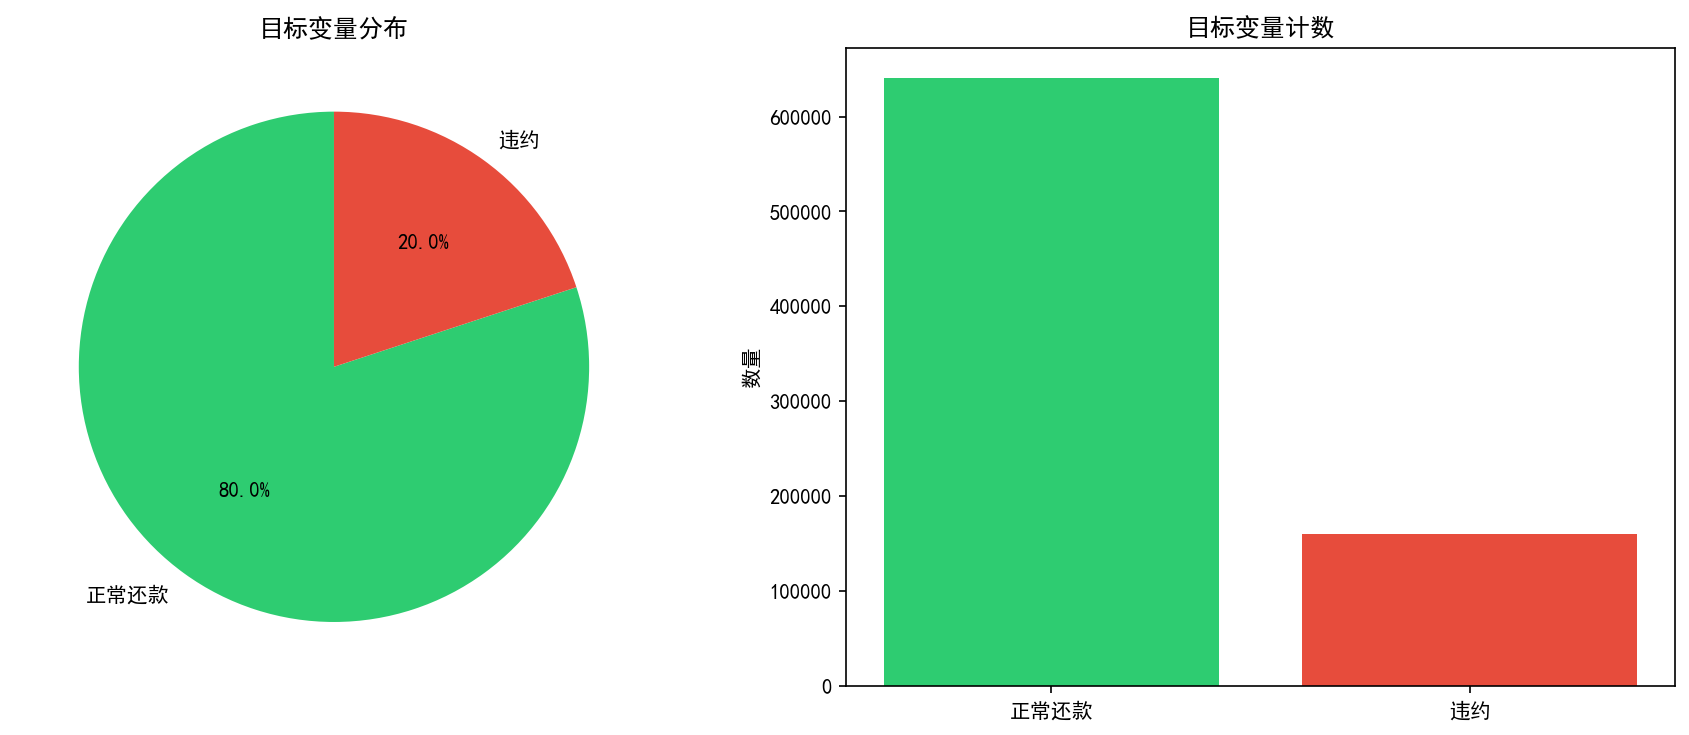
\includegraphics[width=0.82\textwidth]{target_distribution.png}
    \caption{目标变量 isDefault 分布}
    \label{fig:target}
\end{figure}

\subsection{缺失值审计}

缺失值主要集中在 \texttt{n11}、\texttt{employmentLength}、\texttt{n1--n14} 的部分派生字段以及 \texttt{revolUtil} 等变量。缺失比例最高的 \texttt{n11} 约为 8.72\%，仍处于可通过稳健填充处理的范围。图 \ref{fig:missing} 展示了缺失比例最高的特征。

\begin{figure}[H]
    \centering
    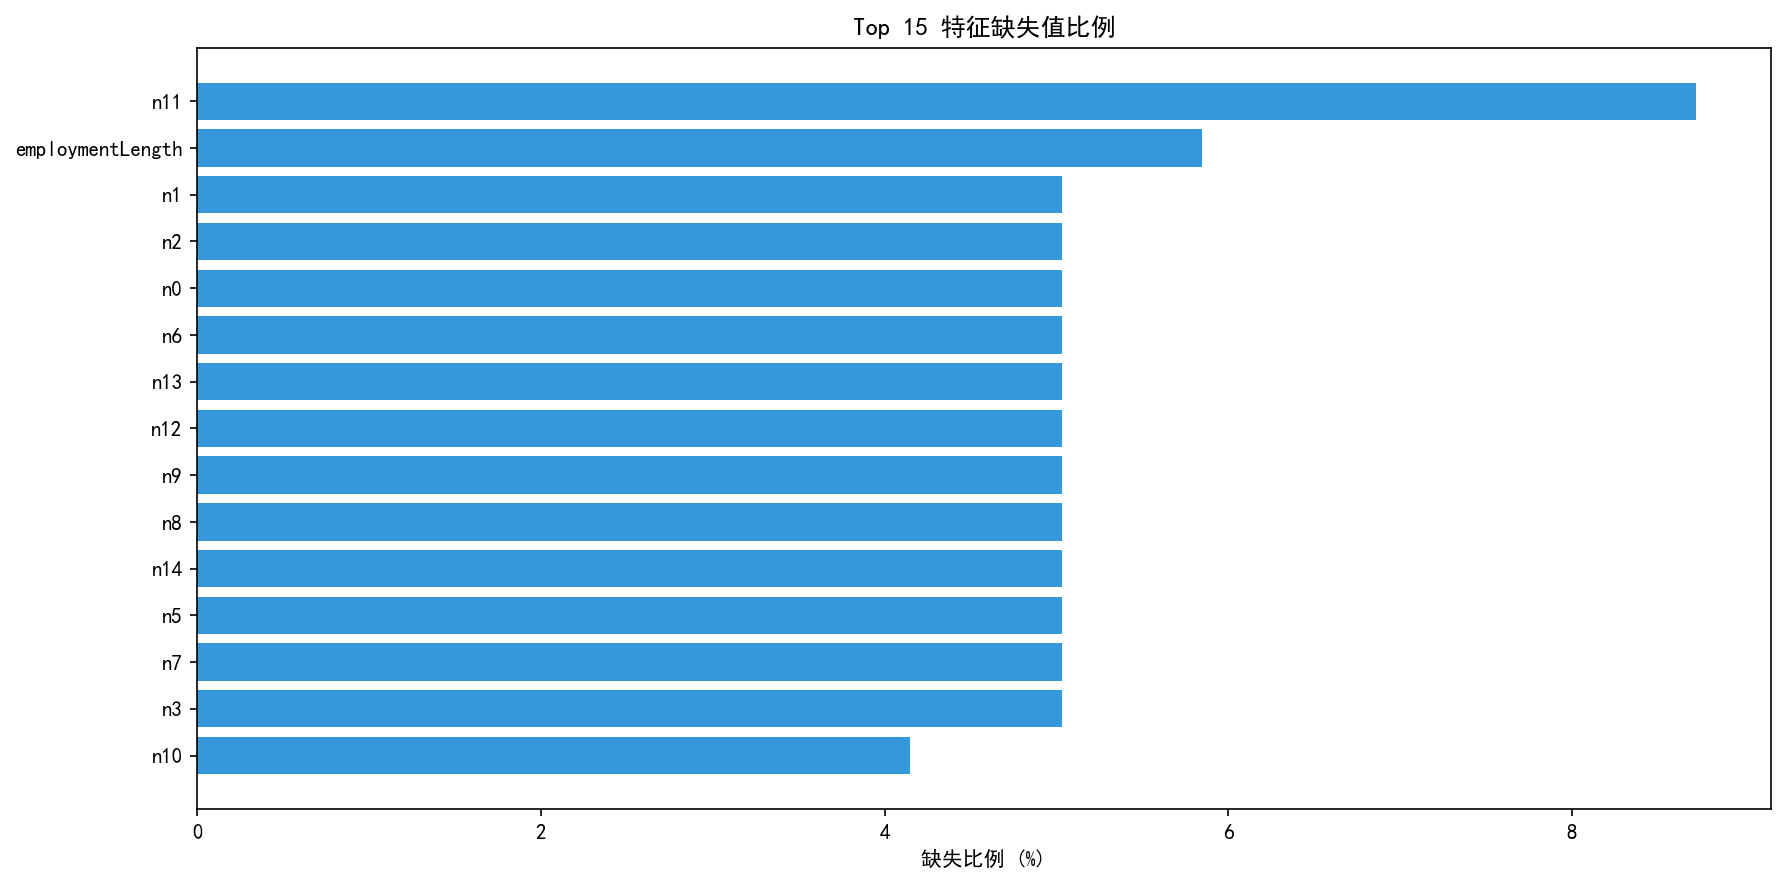
\includegraphics[width=0.88\textwidth]{missing_values.png}
    \caption{主要特征缺失值比例}
    \label{fig:missing}
\end{figure}

为避免数据泄露，缺失值填充只使用建模训练集的中位数，随后将该中位数应用于建模训练集、验证集和测试集。该处理方式保证验证集和测试集不参与任何预处理统计量拟合。

\section{特征预处理与数据隔离}

\subsection{字段清洗与编码}

\texttt{employmentLength} 字段原始值包含“\texttt{< 1 year}”“\texttt{10+ years}”等文本形式，程序将其统一转换为数值型工作年限。\texttt{issueDate} 被拆分为发放年份、月份和星期几，\texttt{earliesCreditLine} 提取最早信用记录年份。

分类变量包括信用等级、住房状态、验证状态、贷款用途、初始列表状态和申请类型等字段。修复后，类别映射仅在建模训练集上拟合；验证集或测试集中未见过的新类别统一映射为“未知类别”编码，避免把验证集或测试集的类别全集提前暴露给模型。

\subsection{训练验证隔离}

本实验最重要的修复之一，是将训练/验证划分提前到预处理和特征筛选之前。修复后的流程为：

\begin{enumerate}
    \item 使用 \texttt{train\_test\_split} 按目标变量分层抽样，先得到建模训练索引和验证索引；
    \item 类别映射、中位数填充、相关性矩阵、IV 筛选均只基于建模训练集拟合；
    \item WOE 分箱和标准化器同样只在建模训练集上拟合；
    \item 交叉验证使用 Pipeline，使每一折都独立拟合 WOE 转换器和标准化器。
\end{enumerate}

这一设计避免了“先看全量训练集再划分验证集”导致的评估偏乐观问题，使验证集 AUC 和 KS 更接近真实样本外表现。

\section{相关性分析与 IV 特征筛选}

\subsection{相关性分析}

模型首先在建模训练集上计算数值特征相关性矩阵，并对相关系数绝对值超过 0.8 的特征对进行冗余剔除。典型高相关特征包括贷款金额与分期金额、FICO 评分上下限、以及若干 \texttt{n} 系列派生变量。对于高相关特征对，程序保留与目标变量 \texttt{isDefault} 相关性更高的一项。

\begin{figure}[H]
    \centering
    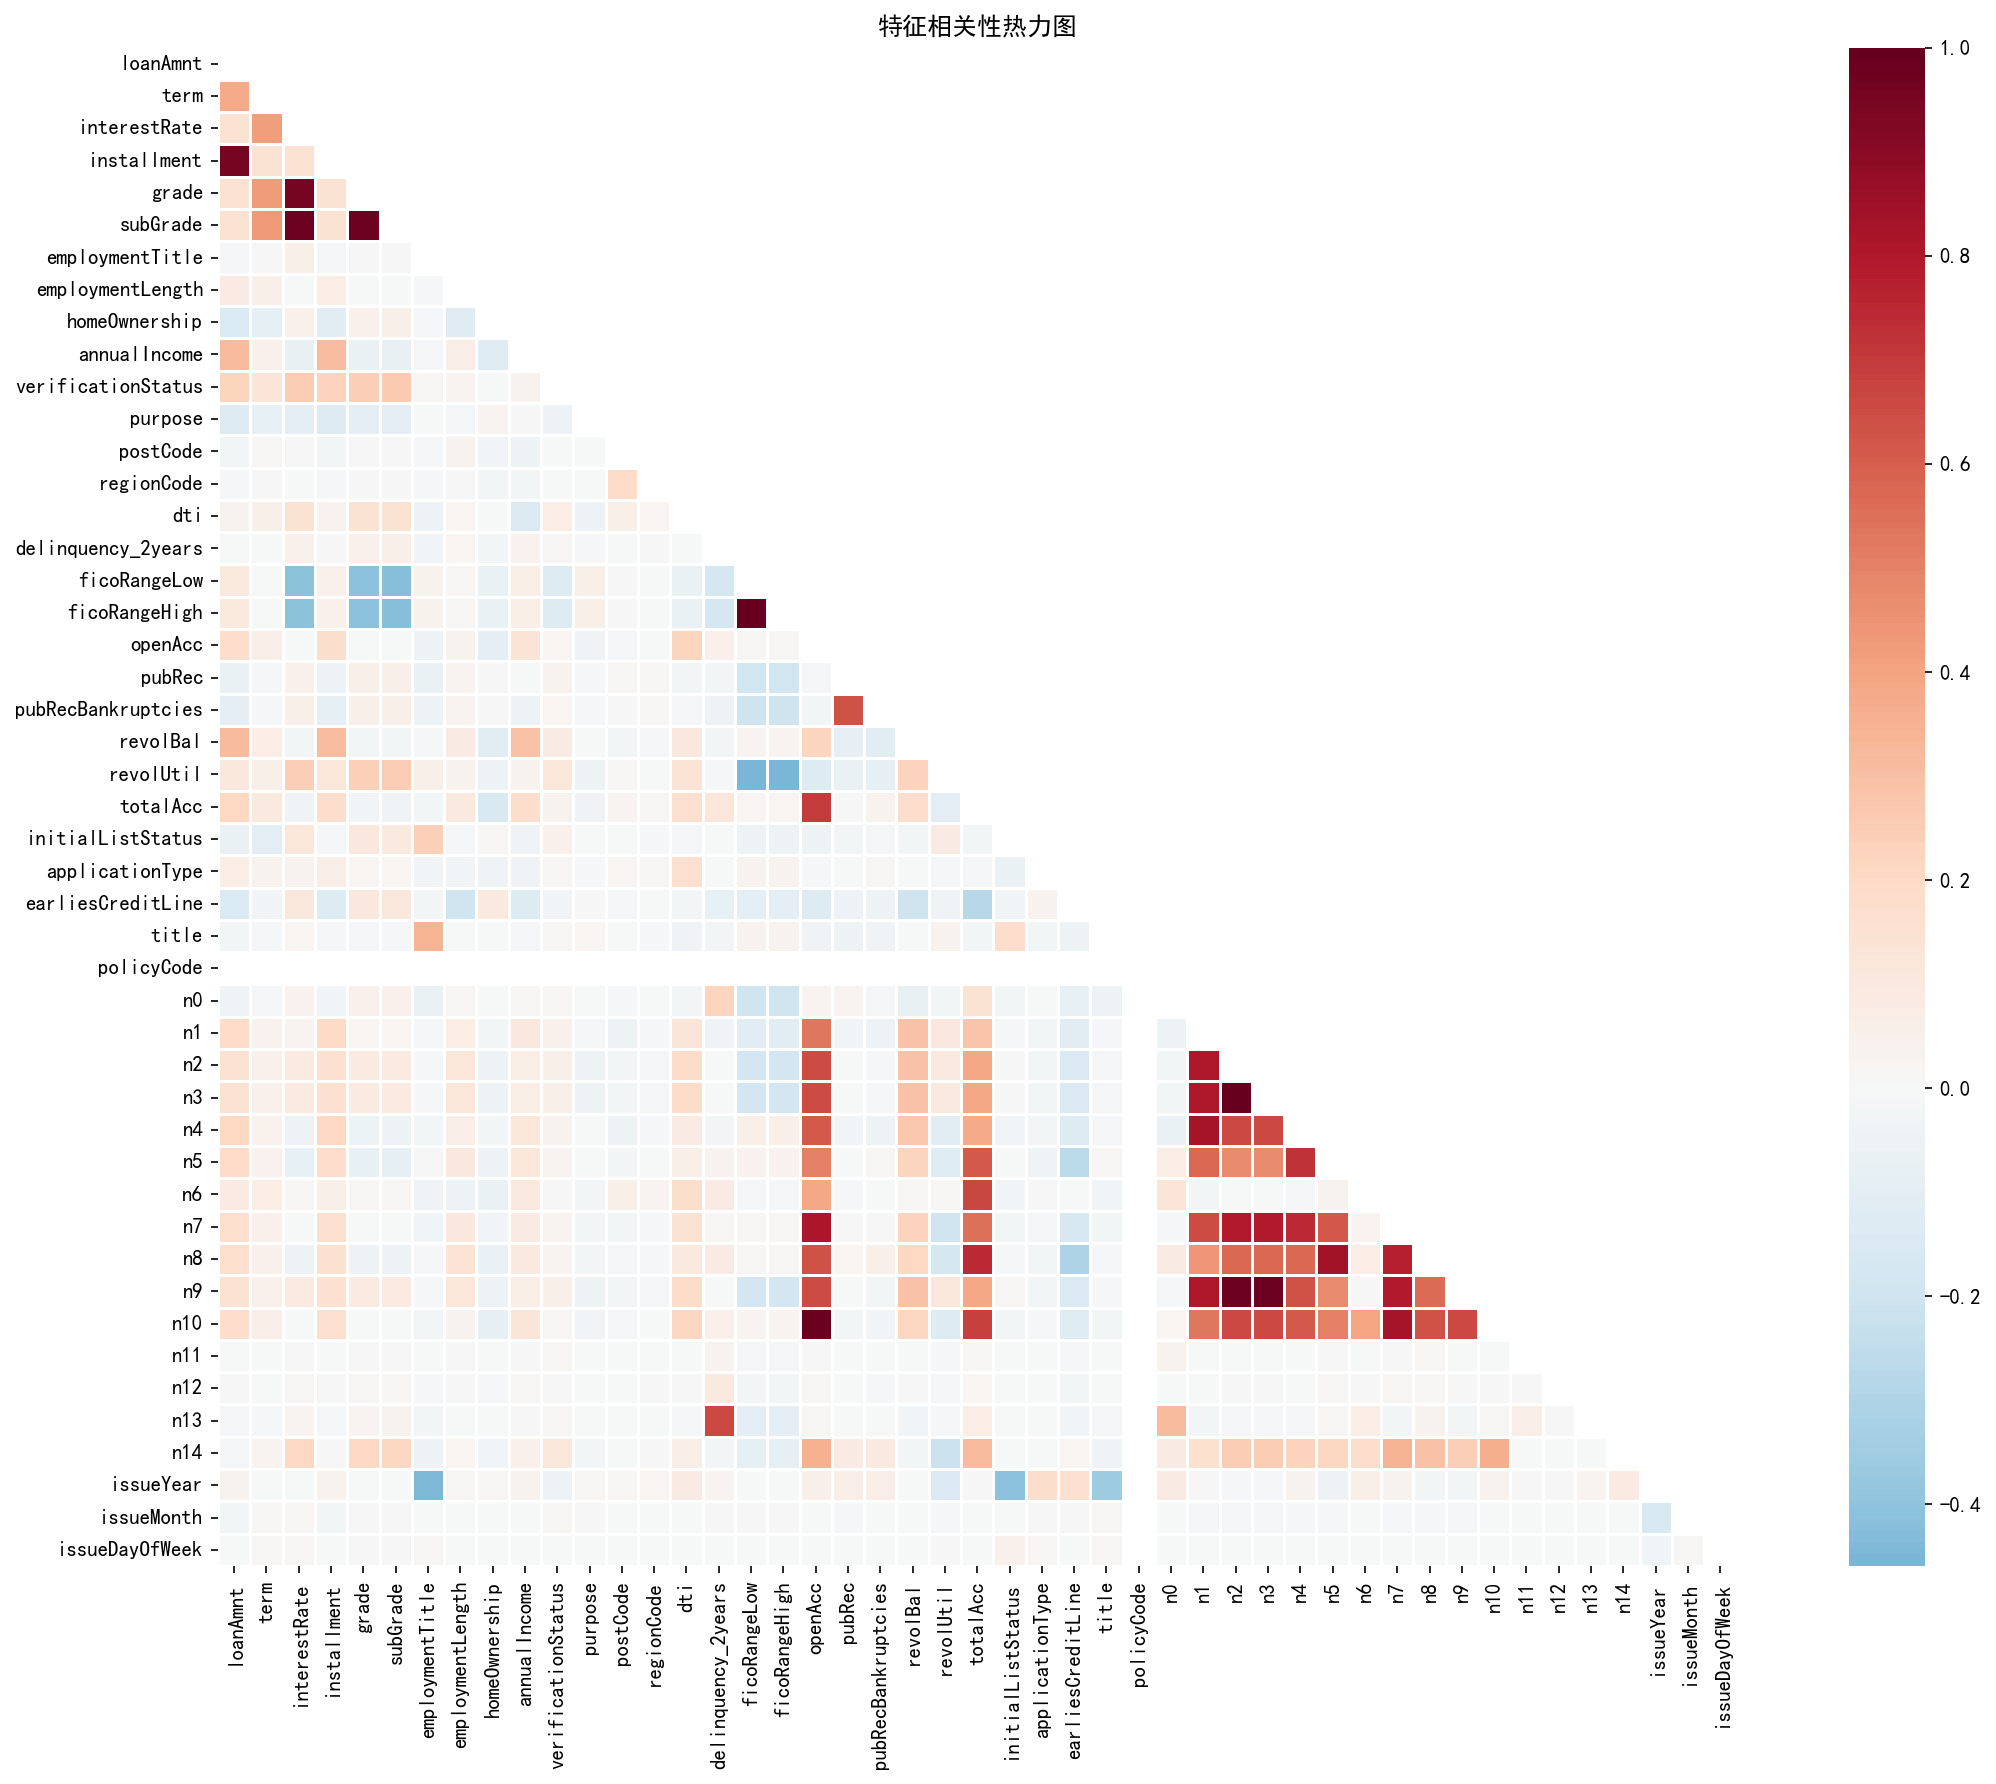
\includegraphics[width=0.96\textwidth]{correlation_heatmap.png}
    \caption{特征相关性热力图}
    \label{fig:corr}
\end{figure}

\subsection{WOE 与 IV 指标}

WOE（Weight of Evidence）用于衡量某一分箱中好样本和坏样本占比的相对差异，定义为：
\begin{equation}
WOE_i=\ln\left(\frac{Good_i/Good_{total}}{Bad_i/Bad_{total}}\right).
\end{equation}

IV（Information Value）用于衡量变量整体区分好坏样本的能力，定义为：
\begin{equation}
IV=\sum_i (GoodPct_i-BadPct_i)\times WOE_i.
\end{equation}

本实验以 IV 不低于 0.02 作为入模阈值，最终选出 11 个有效特征。表 \ref{tab:iv-top} 给出入模特征 IV 值，图 \ref{fig:iv} 展示了 IV 排序。

\begin{table}[H]
    \centering
    \caption{入模特征 IV 值}
    \label{tab:iv-top}
    \begin{tabular}{lrl}
        \toprule
        特征 & IV值 & 预测能力 \\
        \midrule
        subGrade & 0.4868 & 强 \\
        ficoRangeLow & 0.1258 & 中等 \\
        dti & 0.0715 & 弱 \\
        n14 & 0.0428 & 弱 \\
        loanAmnt & 0.0341 & 弱 \\
        issueYear & 0.0337 & 弱 \\
        n2 & 0.0309 & 弱 \\
        annualIncome & 0.0292 & 弱 \\
        verificationStatus & 0.0263 & 弱 \\
        revolUtil & 0.0252 & 弱 \\
        title & 0.0211 & 弱 \\
        \bottomrule
    \end{tabular}
\end{table}

\begin{figure}[H]
    \centering
    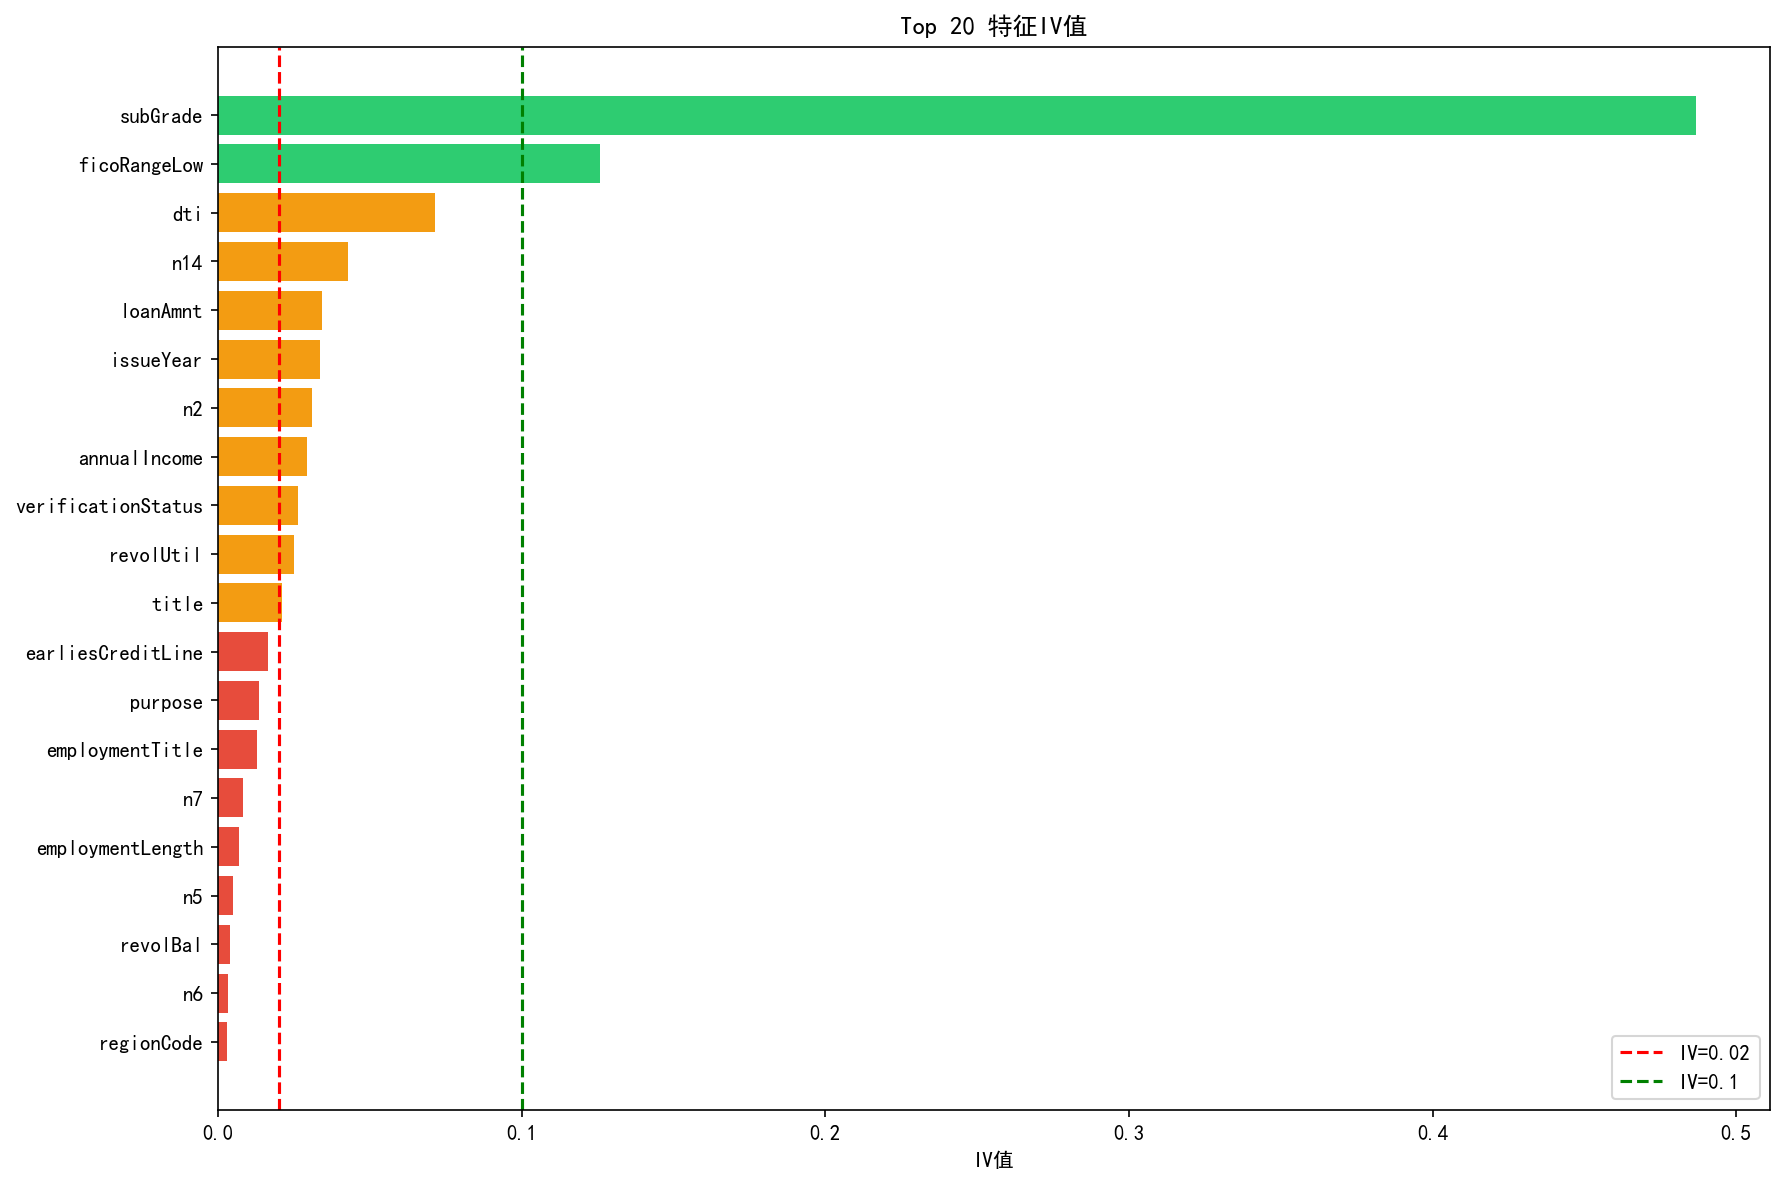
\includegraphics[width=0.88\textwidth]{feature_iv_values.png}
    \caption{特征 IV 值排序}
    \label{fig:iv}
\end{figure}

\section{逻辑回归评分卡建模}

\subsection{WOE 转换与逻辑回归}

信用评分卡强调可解释性和稳定性，因此本实验没有直接将原始数值送入逻辑回归，而是先对入模特征进行分箱，再将各分箱转换为 WOE 值。模型形式为：
\begin{equation}
\ln\frac{p}{1-p}=\beta_0+\beta_1WOE_1+\cdots+\beta_kWOE_k,
\end{equation}
其中 $p$ 表示违约概率。由于 WOE 本身已经体现好坏样本分布差异，逻辑回归系数可以进一步解释各变量在违约风险预测中的方向和强弱。

\subsection{评分卡公式}

模型输出违约概率后，使用标准评分卡公式转换为信用分：
\begin{equation}
Score=Offset+Factor\ln\left(\frac{1-p}{p}\right).
\end{equation}

其中：
\begin{align}
Factor &= \frac{PDO}{\ln 2}=72.13,\\
Offset &= BASE\_SCORE-Factor\ln(BASE\_ODDS)=600.00.
\end{align}

该公式的业务含义是：当好坏比 $(1-p)/p$ 上升时，用户更可能为低风险客户，信用分随之上升。修复前公式方向相反，导致高违约概率对应高信用分；修复后，测试集信用分与违约概率相关系数为 -0.9961，符合“高分低风险”的信用评分常识。

\subsection{标准化评分卡输出}

修复后的 \path{credit_scorecard.csv} 不再只是特征系数表，而是包含 86 行分箱规则。每一行对应某个特征的一个分箱，字段包括特征名、分箱范围、样本数、违约数、正常数、违约率、WOE、IV贡献、特征IV、逻辑回归系数和分箱分数。图 \ref{fig:scorecard-contrib} 展示了评分卡中特征分箱贡献的整体差异。

\begin{figure}[H]
    \centering
    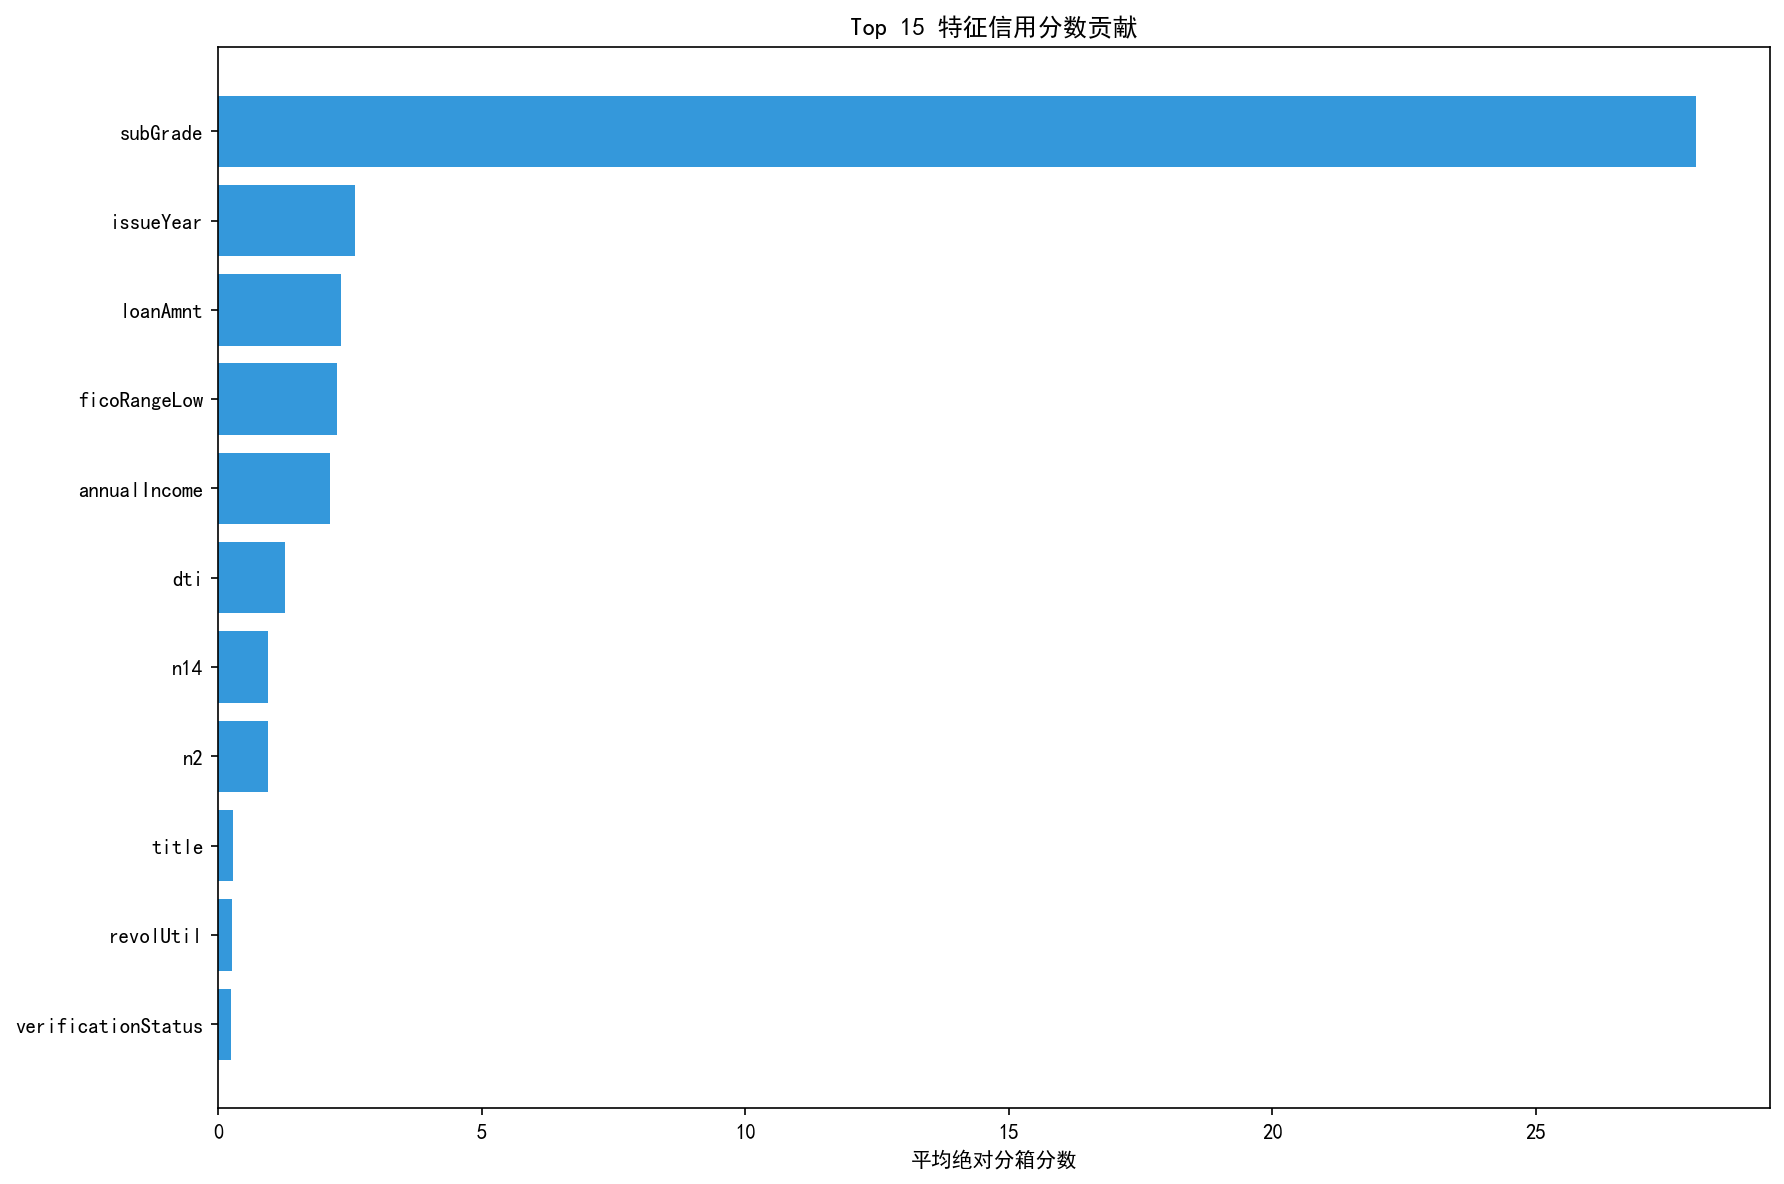
\includegraphics[width=0.88\textwidth]{scorecard_feature_contributions.png}
    \caption{评分卡特征分数贡献}
    \label{fig:scorecard-contrib}
\end{figure}

\section{模型评估结果}

\subsection{交叉验证与验证集指标}

最终模型使用 11 个 IV 筛选后的特征。5 折交叉验证 AUC 为 0.7072，标准差为 0.0021，说明模型在训练样本内部较为稳定。验证集指标如表 \ref{tab:model-metrics} 所示。

\begin{table}[H]
    \centering
    \caption{逻辑回归评分卡模型评估指标}
    \label{tab:model-metrics}
    \begin{tabular}{lr}
        \toprule
        指标 & 数值 \\
        \midrule
        AUC & 0.7058 \\
        KS值 & 0.3006 \\
        准确率 & 0.6304 \\
        精确率 & 0.3079 \\
        召回率 & 0.6833 \\
        F1分数 & 0.4245 \\
        交叉验证AUC均值 & 0.7072 \\
        交叉验证AUC标准差 & 0.0021 \\
        \bottomrule
    \end{tabular}
\end{table}

AUC 超过 0.7，说明模型已经具备基础区分能力；KS 值达到 0.3006，满足风控中约 30\% 的可用参考线。相比单纯追求准确率，风控模型更关注对违约样本的识别能力，因此召回率 0.6833 具有实际意义。

\begin{figure}[H]
    \centering
    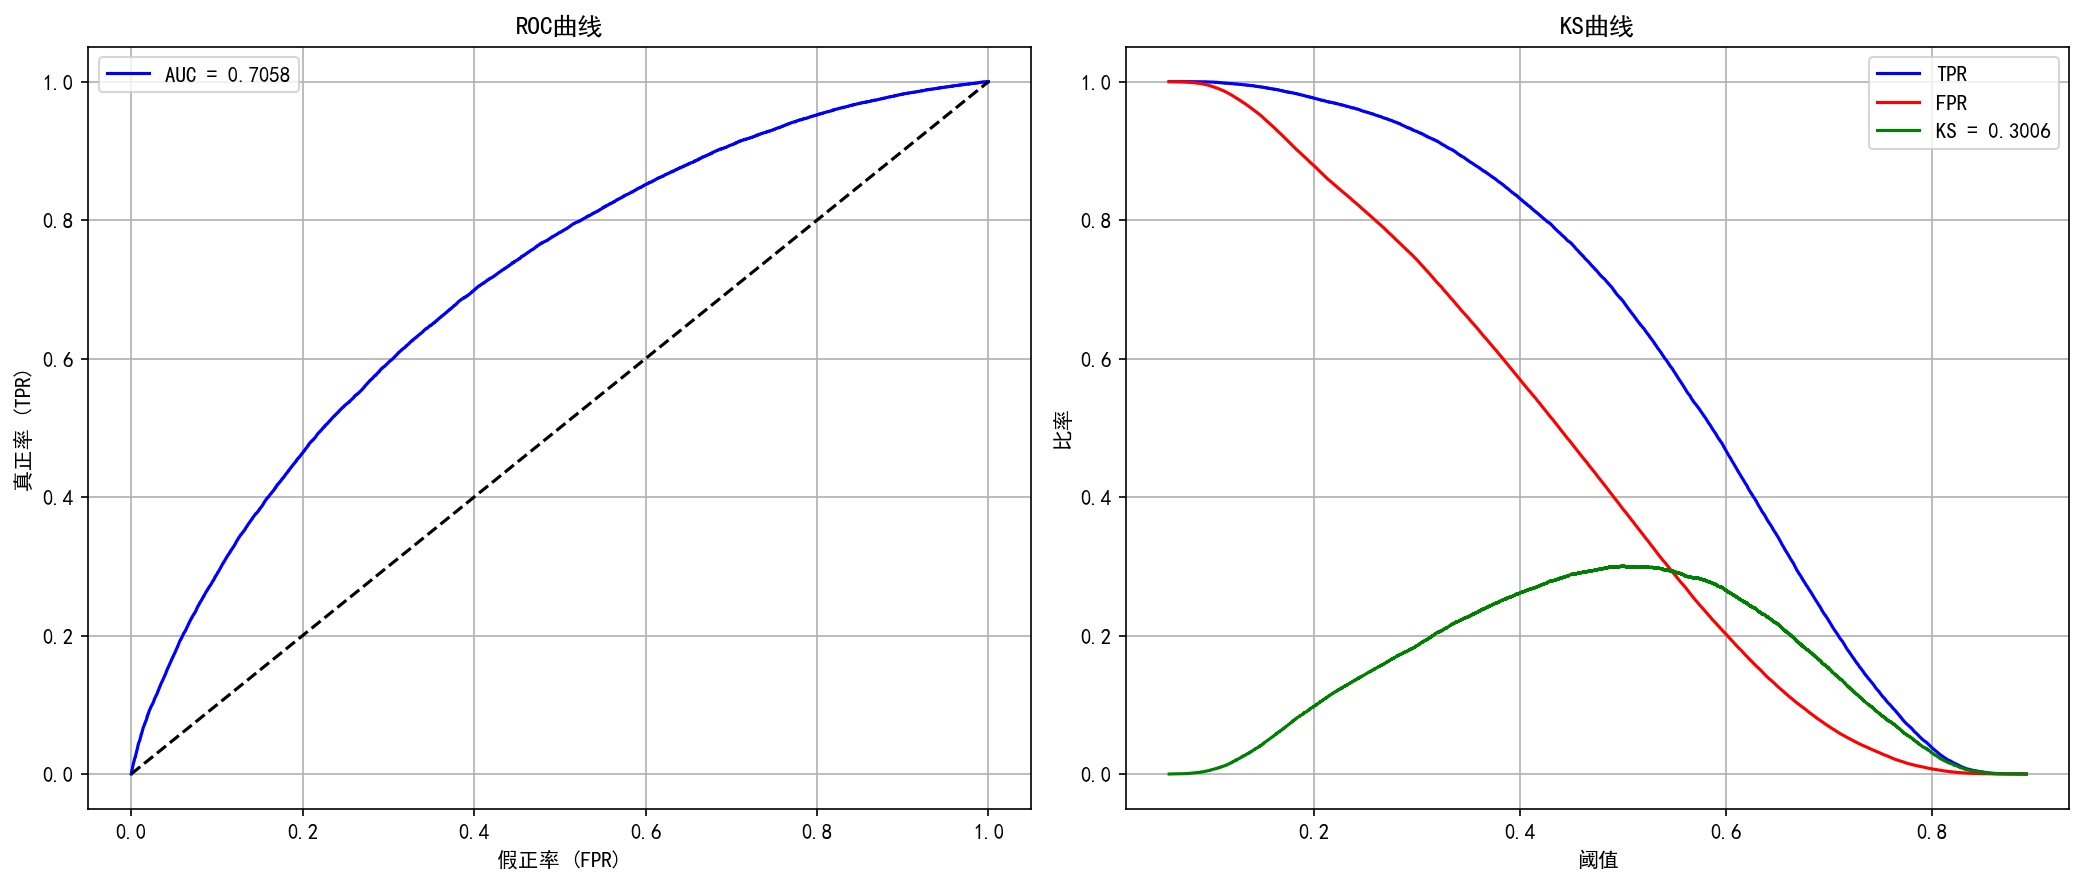
\includegraphics[width=0.92\textwidth]{roc_ks_curves.png}
    \caption{ROC 曲线与 KS 曲线}
    \label{fig:roc-ks}
\end{figure}

\subsection{混淆矩阵}

验证集混淆矩阵如表 \ref{tab:cm} 和图 \ref{fig:cm} 所示。模型识别出 21,812 个真实违约样本，同时仍有 10,110 个违约样本被误判为正常。由于消费金融风控更重视漏判违约用户的风险，后续业务落地时可结合授信策略调整违约阈值。

\begin{table}[H]
    \centering
    \caption{验证集混淆矩阵}
    \label{tab:cm}
    \begin{tabular}{lrr}
        \toprule
        实际/预测 & 预测正常 & 预测违约 \\
        \midrule
        实际正常 & 79,055 & 49,023 \\
        实际违约 & 10,110 & 21,812 \\
        \bottomrule
    \end{tabular}
\end{table}

\begin{figure}[H]
    \centering
    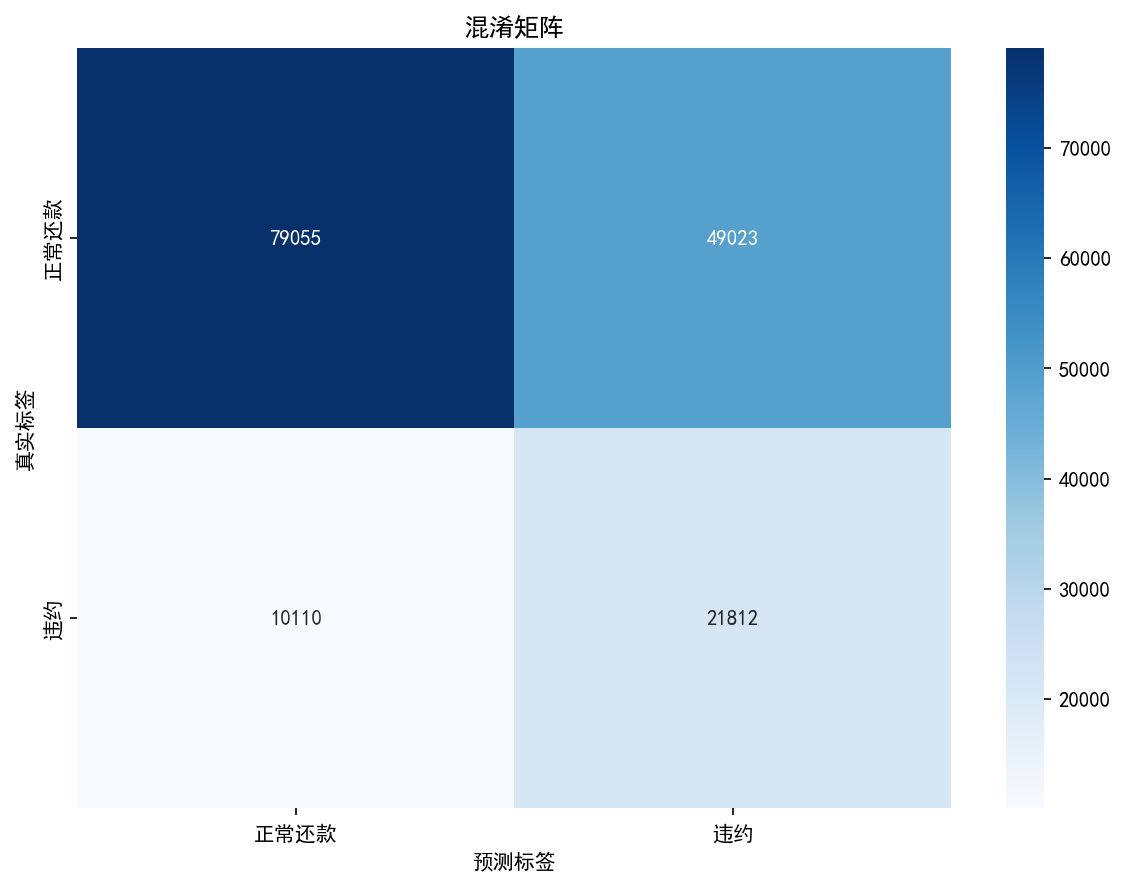
\includegraphics[width=0.70\textwidth]{confusion_matrix.png}
    \caption{混淆矩阵可视化}
    \label{fig:cm}
\end{figure}

\section{特征重要性与金融解释}

\subsection{模型系数重要性}

逻辑回归系数绝对值用于衡量变量对违约概率预测的贡献强度。表 \ref{tab:importance} 展示了全部入模变量的重要性排序，图 \ref{fig:importance} 展示了特征重要性和系数方向。

\begin{table}[H]
    \centering
    \caption{入模特征重要性}
    \label{tab:importance}
    \begin{tabular}{lrr}
        \toprule
        特征 & 重要性 & 系数 \\
        \midrule
        subGrade & 0.6341 & -0.6341 \\
        annualIncome & 0.1993 & -0.1993 \\
        issueYear & 0.1953 & -0.1953 \\
        loanAmnt & 0.1916 & -0.1916 \\
        ficoRangeLow & 0.1054 & -0.1054 \\
        dti & 0.0788 & -0.0788 \\
        n2 & 0.0778 & -0.0778 \\
        n14 & 0.0617 & -0.0617 \\
        title & 0.0286 & 0.0286 \\
        revolUtil & 0.0279 & 0.0279 \\
        verificationStatus & 0.0198 & -0.0198 \\
        \bottomrule
    \end{tabular}
\end{table}

\begin{figure}[H]
    \centering
    
\includegraphics[width=0.96\textwidth]{feature_importance.png}
    \caption{特征重要性与系数方向}
    \label{fig:importance}
\end{figure}

\subsection{核心风险因素解释}

信用子等级是最重要的特征，反映贷款平台已有的信用分层信息；年收入表示收入水平，收入越稳定、越高，偿债能力通常越强；FICO 分数下限是征信质量的重要代理变量；负债收入比直接反映借款人的还款压力；贷款金额越高通常意味着潜在偿付风险和授信风险越大。

从金融逻辑看，模型筛选出的变量与传统信用风险理论一致，说明模型并非依赖无意义的数学组合，而是能够提取收入、负债、信用历史和贷款条件等核心风险信息。

\section{信用评分与等级划分}

\subsection{训练集信用等级}

训练集信用等级统计如表 \ref{tab:train-grade} 所示。除 D 档样本极少外，从 C、B、A 到 S，违约率呈明显下降趋势：C 档违约率为 41.53\%，B 档为 20.51\%，A 档为 7.31\%，S 档为 2.74\%。这说明评分卡方向正确，分数越高，整体违约风险越低。

\begin{table}[H]
    \centering
    \caption{训练集信用等级统计}
    \label{tab:train-grade}
    \begin{tabular}{lrrr}
        \toprule
        信用等级 & 用户数 & 违约数 & 违约率 \\
        \midrule
        D（300--450） & 3 & 1 & 33.33\% \\
        C（450--550） & 116,228 & 48,269 & 41.53\% \\
        B（550--650） & 467,734 & 95,909 & 20.51\% \\
        A（650--750） & 207,963 & 15,210 & 7.31\% \\
        S（750--850） & 8,072 & 221 & 2.74\% \\
        \bottomrule
    \end{tabular}
\end{table}

\subsection{测试集信用评分}

测试集共 200,000 条样本，平均信用分为 613.84，中位数为 608.78，最低分为 445.32，最高分为 797.42。等级分布如表 \ref{tab:test-grade} 所示，主要集中在 B 档和 A 档，少量用户进入 S 档或 D 档。

\begin{table}[H]
    \centering
    \caption{测试集信用等级分布}
    \label{tab:test-grade}
    \begin{tabular}{lr}
        \toprule
        信用等级 & 用户数 \\
        \midrule
        D（300--450） & 2 \\
        C（450--550） & 28,803 \\
        B（550--650） & 117,537 \\
        A（650--750） & 51,660 \\
        S（750--850） & 1,998 \\
        \bottomrule
    \end{tabular}
\end{table}

\begin{figure}[H]
    \centering
    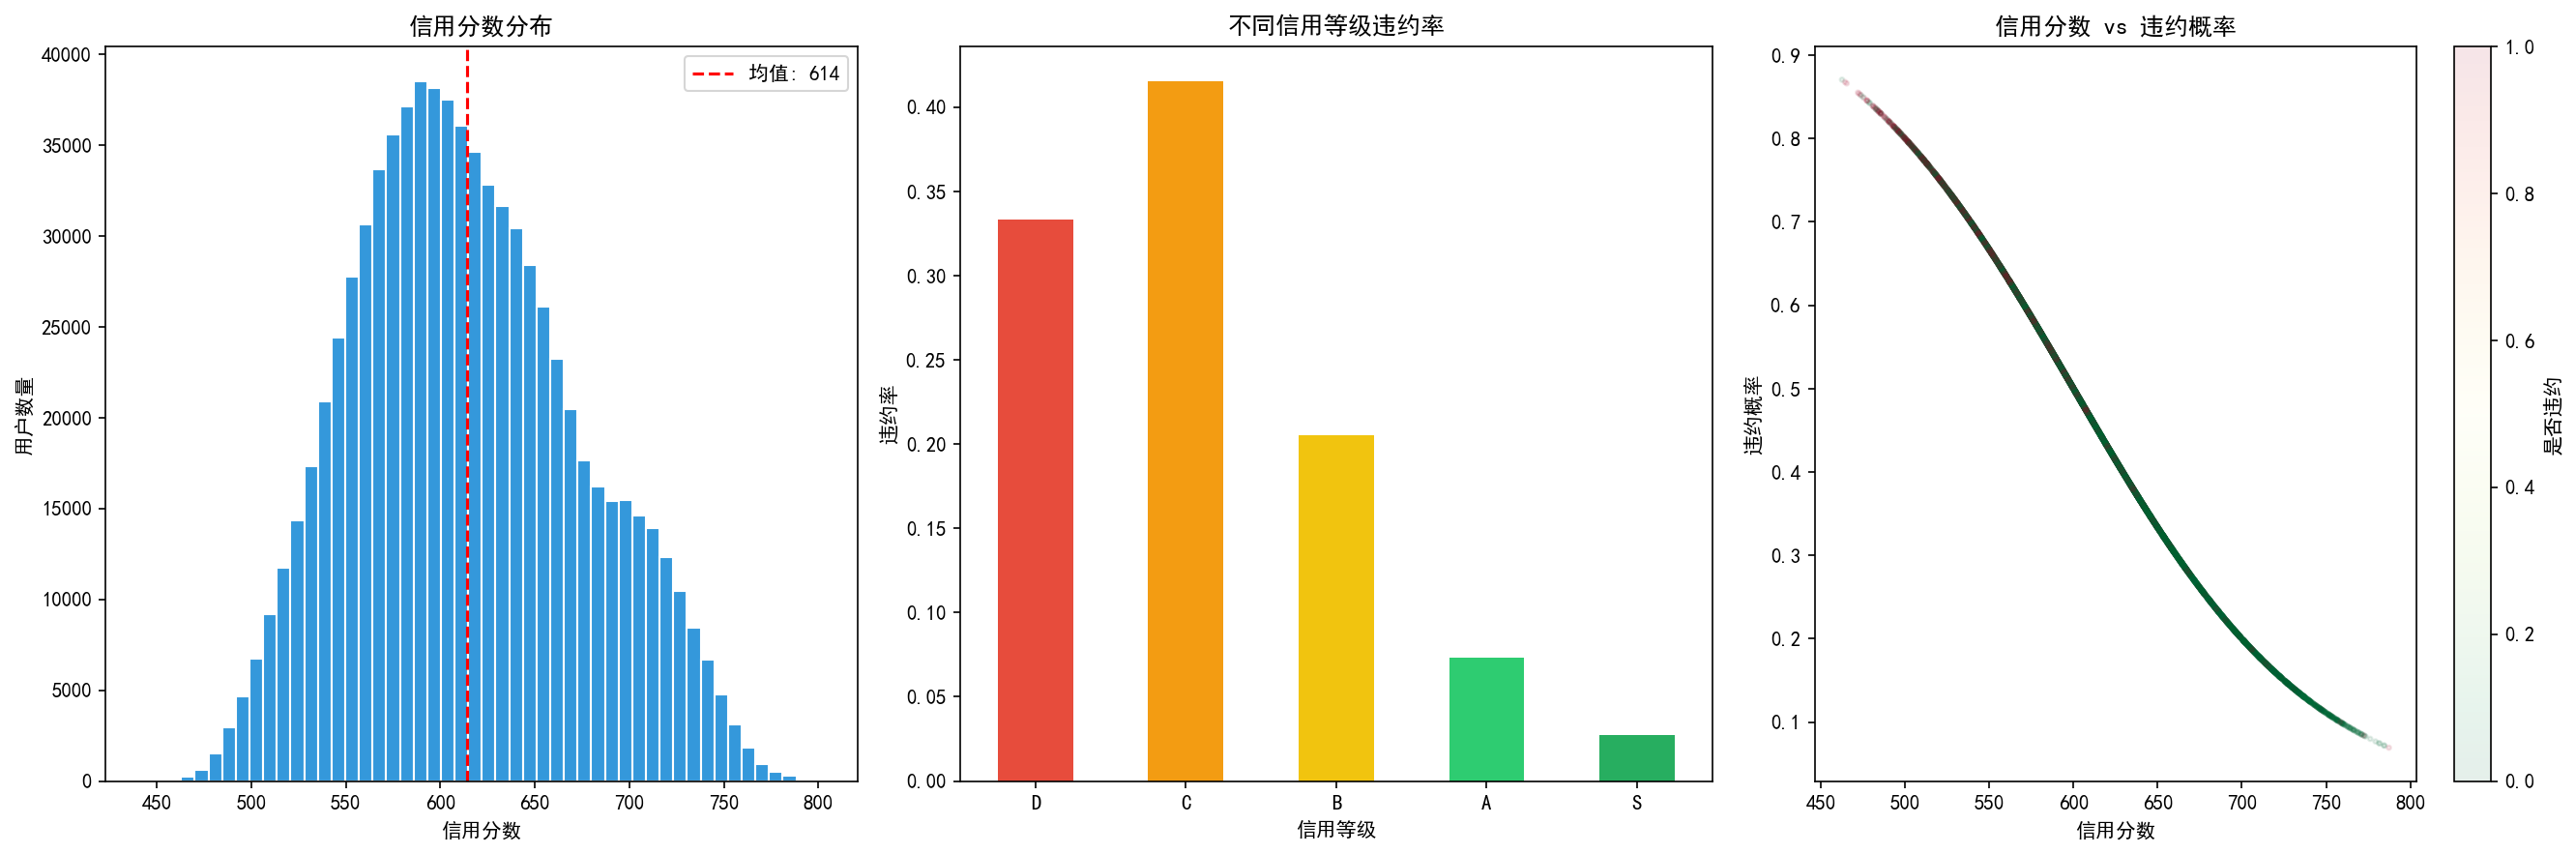
\includegraphics[width=0.98\textwidth]{credit_score_analysis.png}
    \caption{信用分数分布、等级违约率与违约概率关系}
    \label{fig:score-analysis}
\end{figure}

图 \ref{fig:score-analysis} 中，信用分和违约概率呈明显反向关系，测试集相关系数达到 -0.9961。这是本次修复后最关键的业务一致性验证。

\section{信用提升建议}

基于模型结果和评分卡解释，用户提升信用评分可以从以下方面入手：

\begin{enumerate}
    \item 维护良好还款记录，避免逾期和连续逾期，提升信用等级与子等级。
    \item 控制负债收入比，避免超过收入承受能力的借款规模。
    \item 保持稳定收入来源，提高年收入与偿债能力。
    \item 改善征信质量，提高 FICO 评分相关指标。
    \item 控制循环额度使用率，避免长期高比例占用授信额度。
    \item 减少短期内频繁申请信贷，保持稳定信用历史。
\end{enumerate}

从金融机构角度看，评分卡可用于贷前风险筛查、额度分层、定价调整和贷后风险预警。对于 C 档和 D 档用户，应提高审核强度或降低授信额度；对于 A 档和 S 档用户，可给予更高通过率或更优惠利率。

\section{AI代码审查与修复情况}

本次作业额外填写了 AI 代码审查与修复表，主要修复项包括：

\begin{enumerate}
    \item \textbf{信用分方向错误修复：} 修复前信用分公式导致违约概率越高分数越高；修复后改为好坏比越高分数越高。
    \item \textbf{数据泄露风险修复：} 修复前预处理和特征筛选在划分验证集之前完成；修复后先隔离建模训练集和验证集。
    \item \textbf{评分卡规则补强：} 修复前评分卡只有特征系数；修复后输出分箱、WOE、IV贡献和分箱分数。
    \item \textbf{依赖文件补全：} 补充 \texttt{seaborn} 到 \path{requirements.txt}。
    \item \textbf{报告与输出同步：} 重新生成图表、CSV、Markdown 报告和 LaTeX PDF 报告，保证交付物口径一致。
\end{enumerate}

\section{交付物与复现说明}

最终提交材料已整理至“作业十一/提交材料”文件夹，主要文件如表 \ref{tab:deliverables} 所示。

\begin{table}[H]
    \centering
    \scriptsize
    \caption{作业十一提交材料清单}
    \label{tab:deliverables}
    \begin{tabular}{L{0.36\textwidth}L{0.54\textwidth}}
        \toprule
        文件 & 说明 \\
        \midrule
        \path{homework11_credit_scorecard.py} & 完整可运行 Python 源代码 \\
        \path{requirements.txt} & 运行依赖 \\
        \path{credit_scorecard.csv} & 标准化分箱 WOE 信用评分卡 \\
        \path{test_predictions.csv} & 测试集信用分、违约概率和信用等级 \\
        \path{model_evaluation_results.csv} & 模型评估指标 \\
        \path{feature_importance.csv} & 特征重要性结果 \\
        \path{feature_iv_values.csv} & 特征 IV 值结果 \\
        实验报告.md & Markdown 实验报告 \\
        202331060205\_丁致宇\_作业11\_银行信用评分模型报告.pdf & LaTeX 编译 PDF 报告 \\
        AI代码审查与修复表\_作业11\_已填写.docx & 已填写 AI 代码审查与修复表 \\
        AI交互记录.docx & AI 交互记录 \\
        作业11\_代码.zip & 代码压缩包 \\
        作业11\_图表.zip & 图表压缩包 \\
        \bottomrule
    \end{tabular}
\end{table}

复现步骤如下：
\begin{CodeBlock}
pip install -r requirements.txt
python homework11/homework11_credit_scorecard.py
\end{CodeBlock}

运行后将重新生成 \path{outputs/homework11/} 下的全部 CSV 和 PNG 结果。

\section{实验结论}

本实验完成了银行信用评分模型的完整建模与交付流程。最终模型在验证集上取得 AUC 0.7058、KS 0.3006，达到基础风控评分模型的可用水平；评分卡采用 WOE 分箱和逻辑回归，兼具可解释性与可落地性；信用分与违约概率呈显著负相关，测试集相关系数为 -0.9961，说明评分方向正确。

与修复前相比，最终版本不仅能运行，而且在方法上避免了验证集泄露，评分规则也从简单系数表升级为可审查的分箱评分卡。综合来看，本作业已满足“完整可运行代码、特征重要性图表、标准化评分卡、实验报告”的交付要求。

\end{document}
